\documentclass[12pt]{article}
\usepackage[papersize={70cm,100cm},landscape]{geometry}
\usepackage{amsmath}
\usepackage[poster]{tcolorbox}
\pagestyle{empty}
\usepackage{multicol}
\usepackage{xcolor}
\usepackage[hidelinks]{hyperref}

% COLORES UTEC
\definecolor{azulutec}{HTML}{0D2875}
\definecolor{celesteutec}{HTML}{00ADEE}
\definecolor{negro}{HTML}{000000}
\definecolor{blanco}{HTML}{FFFFFF}

\begin{document}
\begin{tcbposter}[
        % opciones para los marcos
        poster={showframe=false, columns=4, rows=6,spacing=10mm},
        % fondo general blanco sin degradado
        coverage={spread, interior style={fill=blanco}},
        % estilo de cajas
        boxes={
                sharp corners=downhill,
                arc=3mm,
                boxrule=1mm,
                colback=blanco,
                colframe=negro,
                title style={
                        left color=celesteutec,
                        right color=celesteutec
                    },
                fonttitle=\bfseries \Huge
            }
    ]

    % -------------------------------
    % COLUMNA 1: Logo UTEC
    \posterbox[blankest,
        halign=center, valign=center,
        interior engine=path,
        interior style={fill=blanco}
    ]{name=logo,column=1,row=1}{
        
\includegraphics[height=9cm]{img/logoUTEC.png}
    }

    % -------------------------------
    % COLUMNAS 2–3: Título centrado
    \posterbox[blankest,
        halign=center, valign=center,
        fontupper=\bfseries\color{azulutec}\huge,
        interior engine=path,
        interior style={fill=blanco}
    ]{name=titulo,column=2,row=1,span=2}{
        \begin{center}
            \resizebox{0.95\linewidth}{!}{\parbox{30cm}{\centering
                    “Optimización de filtros eléctricos en cargadores de baterías\\
                    para vehículos eléctricos mediante la aplicación de funciones de transferencia”
                }}\\[10mm]
            \resizebox{0.6\linewidth}{!}{\textbf{CURSO: ECUACIONES DIFERENCIALES ORDINARIAS}}
        \end{center}
    }

    % -------------------------------
    % COLUMNA 4: Lista de Integrantes
    \posterbox[blankest,
        halign=center, valign=center,
        fontupper=\bfseries\color{azulutec}\huge,
        interior engine=path,
        interior style={fill=blanco}
    ]{name=integrantes,column=4,row=1}{
        \begin{center}
            \textbf{Integrantes:}
            \begin{itemize}
                \item Choque Shuan Katherine Massiel
                \item Huamán Yay Alexis
                \item Oceda Chavez Elizabeth Emperatriz
                \item Vásquez Bustamante María Fernanda
            \end{itemize}
        \end{center}

    }

    % -------------------------------
    \posterbox[adjusted title=Introducción]{name=intro,column=1,row=2, rowspan=1}{
        \huge
        La creciente demanda de vehículos eléctricos ha impulsado el desarrollo
        de cargadores más eficientes y rápidos. Sin embargo, el uso de filtros eléctricos
        tradicionales puede generar distorciones armónicas perjudiciales para la red
        eléctrica. Este proyecto propone optimizar estos filtros mediante el uso de
        funciones de transferencia, lo que permitirá una mejor respuesta dinámica y una
        reducción en la distorción armónica, contribuyendo a la eficiencia energética y
        estabilidad del sistema de carga.

    }
    \posterbox[adjusted title=Objetivos]{name=obj,column=1,row=3, rowspan=2}{
        {\huge
                \textbf{Objetivo general:} \\
                Optimizar el diseño de filtros eléctricos utilizados en cargadores de baterías para vehículos eléctricos, mediante el análisis y aplicación de funciones de transferencia. Esto permitirá mejorar la eficiencia energética, estabilidad operativa y calidad de la energía suministrada durante el proceso de carga.

                \vspace{5mm}

                \textbf{Objetivos específicos:}
                \begin{itemize}
                    \item Analizar el comportamiento dinámico de sistemas de carga con diferentes configuraciones de filtros eléctricos, considerando señales alternas de entrada.
                    \item Evaluar el impacto de las funciones de transferencia en la reducción de distorsiones armónicas y su efecto en la calidad de la señal de salida.
                    \item Comparar el desempeño entre filtros convencionales y optimizados mediante simulaciones matemáticas.
                    \item Proponer un modelo de filtro eléctrico robusto que mejore la eficiencia energética, estabilidad del sistema de carga y que responda adecuadamente ante perturbaciones externas.
                \end{itemize}
            }
    }

    \posterbox[adjusted title=Conclusión]{name=con,column=1,row=5, rowspan=2}{
        {\huge
                El análisis realizado permitió comprender el comportamiento dinámico de los sistemas de carga con filtros eléctricos, validando el modelo matemático propuesto a través de simulaciones precisas.
                Se demostró que los filtros optimizados, basados en funciones de transferencia, reducen eficazmente la distorsión armónica y mejoran tanto la calidad de la energía como la estabilidad del sistema de carga. Esta mejora se evidenció mediante el uso de simulaciones que replican condiciones reales de operación, confirmando así la validez del enfoque teórico propuesto.
                El trabajo integró herramientas analíticas como el uso de la transformada de Laplace y la Ley de Kirchhoff para obtener una solución general al modelo, y luego validó dicha solución frente a resultados numéricos, estableciendo una correlación sólida entre teoría y práctica.
                Desde un punto de vista práctico, los resultados obtenidos tienen impacto directo en la eficiencia energética de los cargadores, al disminuir los armónicos que afectan la transferencia de energía y la vida útil de las baterías. Además, se logró una respuesta estable incluso ante perturbaciones, reflejando un diseño robusto y eficaz.
                En conjunto, este estudio evidencia la relevancia de combinar el análisis matemático riguroso con simulaciones en el desarrollo de tecnologías para la movilidad eléctrica. Proporciona una base sólida para diseñar cargadores más eficientes, sostenibles y confiables, destacando así la importancia de las Ecuaciones Diferenciales como herramienta esencial en la ingeniería moderna.
            }
    }


    \posterbox[adjusted title=Metodología]{name=metod,column=2,span=2,row=2, rowspan=5}{
        \huge
        \begin{multicols}{2}
            \textbf{1. Recolección de datos:} \\
            Se recopilaron parámetros eléctricos reales y teóricos del sistema de carga, incluyendo: resistencia interna de la batería ($R_{bat}$), resistencia equivalente ($R_x$), capacitancia ($C$) e inductancia ($L$). Estos valores fueron esenciales para construir un modelo físico coherente y representativo del sistema bajo estudio.

            \vspace{2mm}

            \textbf{2. Formulación del modelo:} \\
            Se propuso un modelo eléctrico equivalente del sistema de carga. Se consideró una fuente alterna de entrada $v_{in}(t)$ y una variable de estado $q(t)$ que representa la carga acumulada en el condensador.

            \begin{itemize}
                \item Ley de voltajes de Kirchhoff: $\sum V = 0$
                \item Relación corriente-carga: $i(t) = \dfrac{dq(t)}{dt}$
                \item Caída de voltaje en componentes: $V_R = Ri(t), \quad V_C = \dfrac{q(t)}{C}$
            \end{itemize}

            Se obtuvo el siguiente modelo diferencial de primer orden:
            \[
                (R_{bat} + R_x + R_L) \frac{dq(t)}{dt} + \frac{q(t)}{C} = v_0 \sin(\omega t)
            \]

            \vspace{1mm}
            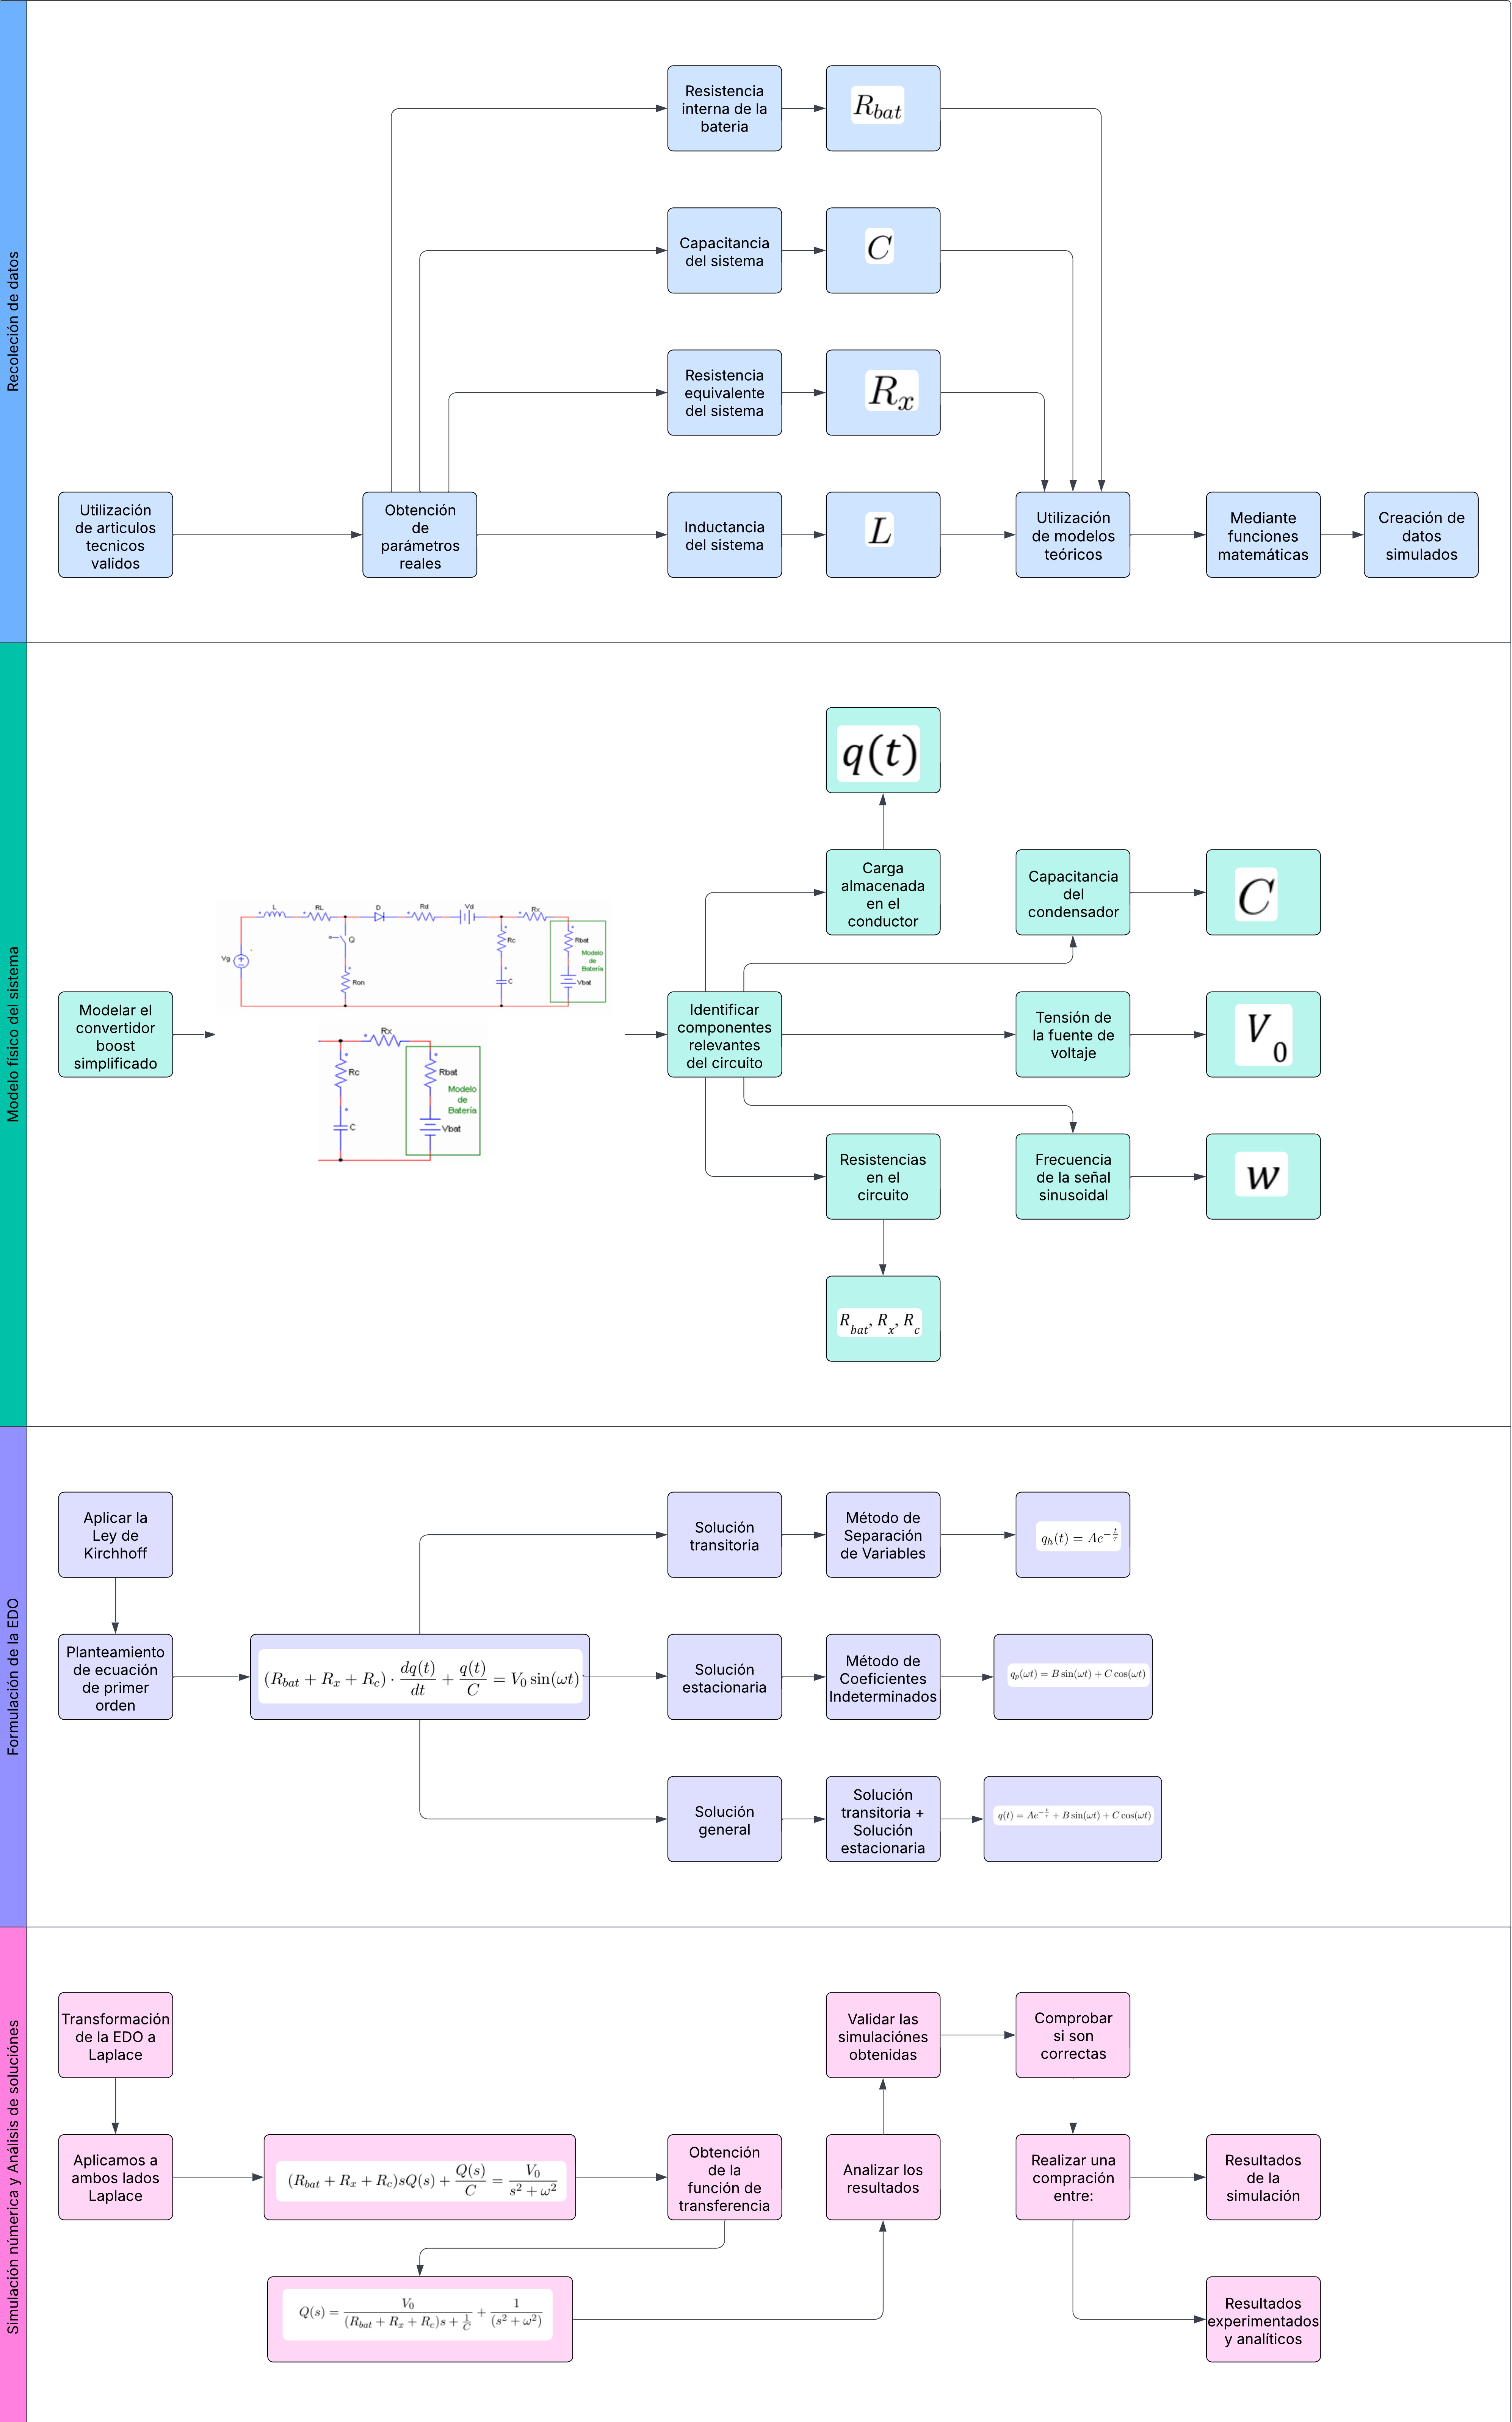
\includegraphics[width=\linewidth, height=1000pt]{img/diagrama.png}
            \vfill
            \columnbreak
            \textbf{3. Justificación del enfoque analítico:}
            \begin{itemize}
                \item \textbf{Precisión:} permite describir el comportamiento exacto del sistema.
                \item \textbf{Adecuación:} se ajusta al tipo de entrada y parámetros.
                \item \textbf{Comprensión:} permite interpretar los efectos de cada parámetro.
                \item \textbf{Ventajas:} genera una función de transferencia útil para el análisis dinámico.
            \end{itemize}

            \vspace{2mm}

            \textbf{4. Procedimiento analítico:} \\
            Se aplicaron métodos de solución de EDOs. Tras plantear el modelo, se utilizó la transformada de Laplace para obtener la función de transferencia:

            \[
                \mathcal{L}\left\{(R_{bat} + R_x + R_L)\frac{dq(t)}{dt} + \frac{q(t)}{C}\right\} = \mathcal{L} \left\{v_0 \sin(\omega t)\right\}
            \]

            \[
                Q(s) = \frac{v_0 \cdot \omega}{\left[(R_{bat} + R_x + R_L)s + \frac{1}{C}\right](s^2 + \omega^2)}
            \]

            \vspace{2mm}

            Además, se resolvió la EDO en el dominio del tiempo aplicando el método de coeficientes indeterminados, obteniéndose la solución general como suma de la solución homogénea y particular:

            \[
                q(t) = q_h(t) + q_p(t)
            \]

            Donde la solución homogénea es:

            \[
                q_h(t) = Ae^{-\frac{t}{\tau}} \quad \text{con} \quad \tau = \frac{C}{R_{bat} + R_x + R_L}
            \]

            Y la solución particular:

            \[
                q_p(t) = B \sin(\omega t) + C \cos(\omega t)
            \]

            Por lo tanto, la solución general del sistema es:

            \[
                q(t) = Ae^{-\frac{t}{\tau}} + B \sin(\omega t) + C \cos(\omega t)
            \]

            Esta solución refleja el comportamiento dinámico del sistema considerando tanto el régimen transitorio (término exponencial) como el estacionario (respuesta sinusoidal).

            \textbf{5. Limitaciones del enfoque:} \\
            El modelo analítico, si bien preciso, supone condiciones ideales:
            \begin{itemize}
                \item No contempla pérdidas térmicas ni conmutaciones no lineales.
                \item No incorpora el comportamiento dependiente del tiempo de algunos materiales.
                \item La respuesta es teórica; se valida luego numéricamente.
            \end{itemize}

        \end{multicols}
    }



    \posterbox[adjusted title=Resultados]{name=res,column=4,row=2, rowspan=4}{
        \huge
        Se obtuvo la \textbf{respuesta dinámica} del sistema de carga ante una señal alterna tipo seno, aplicando los parámetros óptimos obtenidos durante el desarrollo analítico. Los resultados permiten evaluar con claridad cómo el comportamiento del sistema mejora al incorporar un filtro diseñado cuidadosamente. En particular, se evidencia que el sistema responde de forma controlada y sostenida, sin picos abruptos ni efectos transitorios persistentes. Esto demuestra que el filtro optimizado no solo \textbf{reduce significativamente la distorsión armónica}, sino que también contribuye a una notable mejora en la \textbf{estabilidad del sistema} y su desempeño frente a perturbaciones.

        \vspace{2mm}

        La Figura 1 muestra cómo la señal alterna aplicada genera una \textbf{respuesta oscilatoria suave y estable} en la carga almacenada del condensador. Esta respuesta representa el comportamiento estacionario del sistema y valida la solución particular obtenida de la EDO.
        La Figura 2 presenta el \textbf{espectro de frecuencias} de la señal de salida, mostrando un claro dominio de la frecuencia fundamental y una considerable reducción en componentes armónicas no deseadas, lo que indica una alta calidad del filtrado.

        \vspace{2mm}

        Ambas gráficas evidencian que el modelo analítico no solo predice adecuadamente el comportamiento del sistema, sino que al ser comparado con simulaciones confirma su validez en situaciones prácticas. En particular:

        \begin{itemize}
            \item La respuesta a la entrada senoidal sigue el perfil esperado del sistema RLC, sin sobrepasos abruptos ni inestabilidades.
            \item El sistema demuestra una rápida estabilización incluso ante perturbaciones, lo cual indica un diseño de filtro eficaz.
            \item La función de transferencia implementada logra una excelente \textbf{atenuación de armónicos}, esencial para preservar la calidad energética del cargador.
        \end{itemize}

        \vspace{2mm}

        \begin{minipage}[t]{0.49\textwidth}
            \centering
            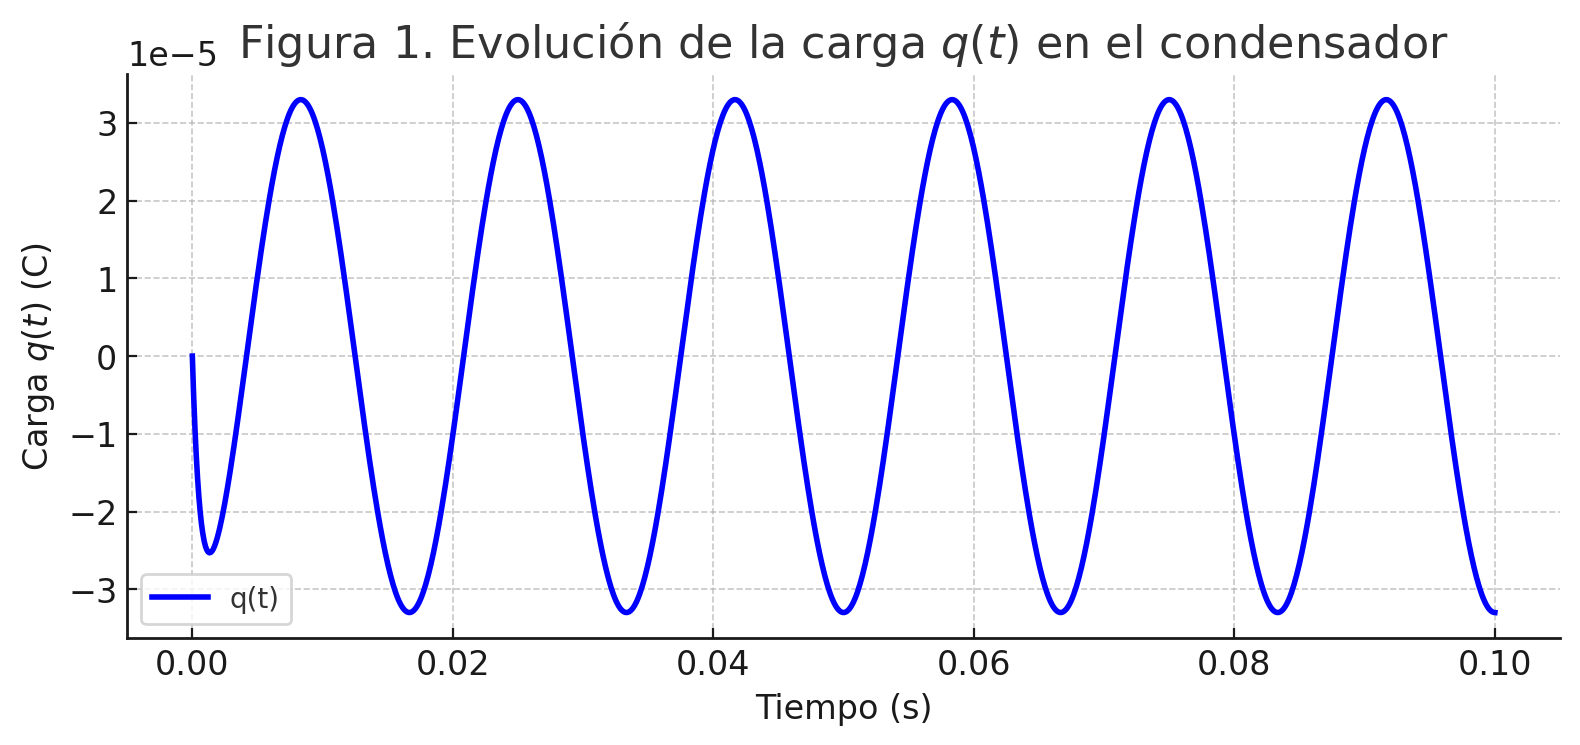
\includegraphics[width=\linewidth]{img/7.png}\\
            \textbf{Figura 1.} Respuesta a entrada senoidal
        \end{minipage}
        \hfill
        \begin{minipage}[t]{0.49\textwidth}
            \centering
            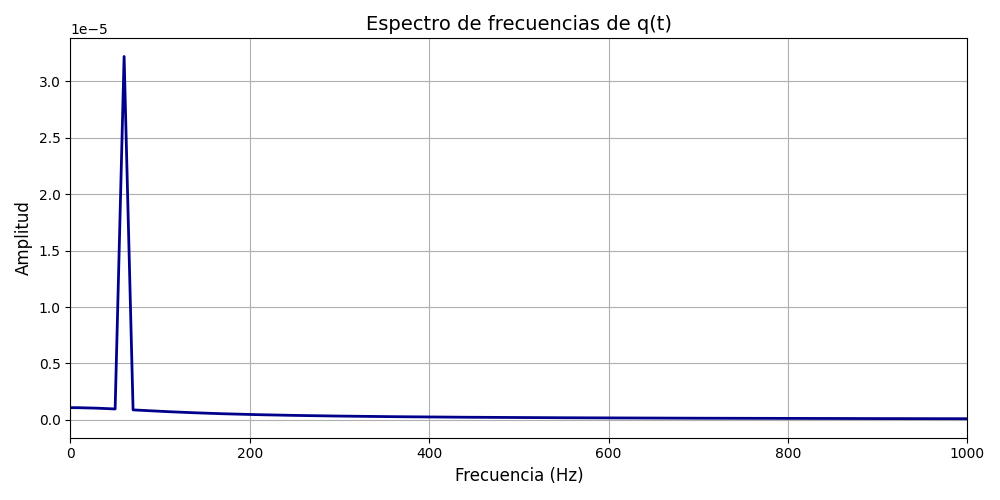
\includegraphics[width=\linewidth]{img/8.png}\\
            \textbf{Figura 2.} Estabilidad ante perturbación
        \end{minipage}

    }


    \posterbox[adjusted title=Bibliografía]{name=biblio,column=4,row=6}{
        \large
        \textbullet\ Abundis, A. (2016). *Causas y efectos de armónicos en sistemas eléctricos de potencia*. Universidad Nacional Autónoma de México, Facultad de Ingeniería. \url{http://132.248.52.100:8080/xmlui/handle/132.248.52.100/11159}\par\medskip
        \textbullet\ Paipa, C. C., Ramirez, J. C., Trujillo R., C. L., Alarcón V., J. A., \& Jaramillo M., A. A. (2020). *Battery charger design with low current harmonic distortion for application in electric vehicles*. Ingeniare. Revista chilena de ingeniería, 28(4), 706–717. \url{https://dx.doi.org/10.4067/S0718-33052020000400706}\par\medskip
        \textbullet\ Cittanti, D., Mandrile, F., \& Bojoi, R. (2021). *Design Space Optimization of a Three-Phase LCL Filter for Electric Vehicle Ultra-Fast Battery Charging*. Energies, 14(5), 1303. \url{https://doi.org/10.3390/en14051303}
    }

\end{tcbposter}
\end{document}
